% Copyright (C)  2015  Alexander Jankowski, Philipp Hacker.
% Permission is granted to copy, distribute and/or modify this document
% under the terms of the GNU Free Documentation License, Version 1.3
% or any later version published by the Free Software Foundation;
% with no Invariant Sections, no Front-Cover Texts, and no Back-Cover Texts.
% The lincense itself can be found at <https://www.gnu.org/licenses/fdl-1.3>.

\documentclass[numbers=noenddot,a4paper,notitlepage,twoside,BCOR15mm]{scrartcl}
%\documentclass[numbers=noenddot,12pt,a4paper]{scrartcl}

\usepackage{ifoddpage}
\usepackage[infoshow]{tabularx}
\usepackage{fancyhdr}
\usepackage[greek,ngerman]{babel}
\usepackage[T1]{fontenc}
\usepackage[utf8]{inputenc}
\usepackage{libertine}
\usepackage{ziffer}
\usepackage{graphicx}
\usepackage{units}
\usepackage[infoshow]{tabularx}
\usepackage[all]{xy}
\usepackage{amsmath}
\usepackage{amssymb}
\usepackage{wrapfig}
\usepackage{upgreek}
\usepackage{esint}
\usepackage{float}
\usepackage[font=small,labelfont=bf]{caption}
\usepackage{subcaption}
\usepackage{lscape}
\usepackage[backref=page]{hyperref}
\usepackage{cleveref}
\usepackage{csquotes}

\renewcommand{\headrulewidth}{0.1pt}
\renewcommand{\footrulewidth}{0.1pt}
\newcommand{\name}{\text{Philipp Hacker}} %TODO Name des Protokollanten eintragen

\renewcaptionname{ngerman}{\figurename}{Abb. }
\renewcaptionname{ngerman}{\tablename}{Tab.}

\setlength{\parindent}{0pt}

\newcommand{\nummat}[1]{\left[\text{#1}\right]}
\newcommand{\num}[1]{$\left[\text{#1}\right]$}
\newcommand{\degree}{^\circ}
\newcommand{\diff}{\textnormal{d}}
\newcommand{\tenpo}[1]{ 10^{#1}}
\newcommand{\greek}[1]{\greektext#1\latintext}
\newcommand{\ix}[1]{_\text{#1}}
\newcommand{\imag}{\mathbf{i}}
\newcommand{\tilt}[1]{\textit{#1}}
\newcommand{\grad}[1]{\textit{grad}\left(#1\right)}
\newcommand{\divergenz}[1]{\textit{div}\left(#1\right)}
\newcommand{\euler}{\mathnormal{e}}
\newcommand{\fett}[1]{\textbf{#1}}
\newcommand{\einnup}{\hspace{0.2cm}}
\newcommand{\einnum}{\hspace{-0.2cm}}
\newcommand{\zentriert}[1]{\begin{center}#1\end{center}}
\newcommand{\OP}[1]{\hat{\mathrm{#1}}}

\title{Protokoll: OH-Rotationsspektroskopie} %TODO Name des Versuchs eintragen
\author{Alexander Jankowski, Philipp Hacker}
\date{\today}
\pagestyle{fancy}
\fancyhead[C]{\thepage}
\fancyhead[R]{\name}
\fancyfoot[C]{\thepage}
\fancyhead[L]{Abschnitt \thesection}

\begin{document}
	\maketitle
	\begin{center}
		Betreuer: Sebastian Runde\\ %TODO Name des Betreuers eintragen
		Versuchsdatum: 11.11.2015\\ %TODO Datum des Versuchs eintragen
		\begin{table}[h]
			\centering
			Note: %TODO Gute Note erhalten :)
			\begin{tabularx}{1.5cm}{|X|}
				\hline \\ \\
				\hline
			\end{tabularx}
		\end{table}
	\end{center}
	\vspace*{\fill}
	\tableofcontents
	\vfill
	\newpage
	\section{Motivation}

		Mit der Theorie zur Beschreibung quantenmechanischer Übergänge auf atomarer und molekularer Ebene ist es möglich, die Thermodynamik höherer Atmosphärenschichten vom Boden aus zu untersuchen. Die theoretische Physik liefert hierbei die Vorschrift für die Auswertung der Intensitätsmaxima auf kleinsten Wellenlängenintervallen, vorausgesetzt man hat Kenntnis über die Probensubstanzen entlang der Sichtlinie. Anhand dieses Versuchs soll das Prinzip der Temperaturbestimmung in der Mesopause - mit Hilfe von Rotationszuständen im großkanonischen Ensemble der Atmosphärenschicht - nachvollzogen werden.

	\newpage
	\section{Physikalische Grundlagen}

			\begin{figure}[b]
				\centering
				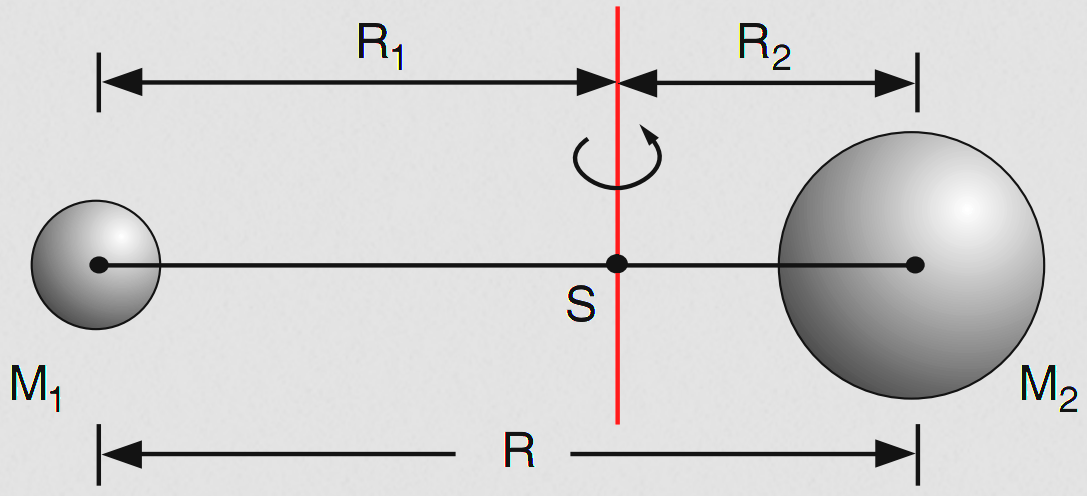
\includegraphics[width=0.6\textwidth]{molekulrotat.png}
				\caption{Schema eines Moleküls zweier verschiedener Monomere.}
				\label{img:molekul}
			\end{figure}

		In der Temperaturmessung höherer Atmosphärenschichten - wie der Mesosphäre/-pause in diesem Falle -  macht man sich Spektren quantenmechanischer Übergängen von Molekülen und/oder Atomen zu Nutze. Insbesondere die durch elektromagnetische Strahlung, e.g. Sonnenwind, im sogenannten \tilt{Airglow} angeregten Übergänge können mit Hilfe von Gitterspektrographen gut untersucht werden.\\
		Die quantenmechanische Grundlage für das Verständnis der Spektren liegt in der \tilt{stationären Schrödinger-Gleichung} \autoref{eq:schr} für die Orbitale des Moleküls $\fett{A}\ix{1}\fett{A}\ix{2}$, wobei $\fett{A}\ix{1}$ und $\fett{A}\ix{2}$ die Monomere der zu untersuchenden Spezies sind. Man setzt im Bild des \tilt{Starren Rotators} mit $M$ die reduzierte Masse des Systems und mit $\Omega$ deren gemeinsames Trägheitsmoment bezüglich einer Achse durch den Molekülschwerpunkt an.\\
		In \autoref{eq:schr} nutzt man einen Separationsansatz für die schnellen Elektronen $\Psi_{e,\lambda}^{(0)}$ und trägen Kerne $\Phi_{K,\lambda}$ aus, welcher auf der \tilt{Born'schen Näherung} beruht. Von Interesse ist hierbei der Anteil für die Nuklei, welcher das Ergebnis aus \autoref{eq:hamilt} hat. Hier ist mit $\lambda$ ein Satz von Quantenzahlen mit $J$ der Rotationsquantenzahl, $\vec{R\ix{i}}$ eine Kernposition im Schwerpunktsystem, $\vec{r\ix{j}}$ ein Elektronen-Vektor und $R$ der Kernabstand bezeichnet.

			\begin{align}
				\left(-\frac{\hbar^2}{2M\ix{1}}\Delta\ix{1}-\frac{\hbar^2}{2M\ix{2}}\Delta\ix{2}+V(\vec{R\ix{i}},\lambda)\right)\Theta&(\vec{r\ix{j}},\vec{R\ix{i}})=\left(E_{e,\lambda}+E_{K,\lambda}\right)\Theta(\vec{r\ix{j}},\vec{R\ix{i}}) \label{eq:schr}\\
				\Theta(\vec{r\ix{j}},\vec{R\ix{i}})=\Phi_{K,\lambda}&(\vec{R\ix{i}})\Psi_{e,\lambda}^{(0)}(\vec{r\ix{j}},\vec{R\ix{i}}) \nonumber \\
				\OP{H}\ix{K}\Phi_{K,\lambda}=E\ix{rot}\Phi_{K,\lambda}=&\frac{\hbar^2J\left(J+1\right)}{2MR^2}\Phi_{K,\lambda}=\frac{\vec{J}^2}{2\Omega}\Phi_{K,\lambda} \label{eq:hamilt}
			\end{align}

		Die Energie-Eigenwerte des \tilt{Hamilton-}Operators sind die Niveaus der Rotationszustände des in \autoref{img:mole} gezeigten Moleküls. Diese sind diskrete Werte, deren Abstand mit der Gesamt-Rotationszahl $J$ größer wird. Aus der \autoref{eq:hamilt} erhält man die Auswahlregel $\Delta J=0,\pm1$ zwischen zwei Energie-Niveaus. Diese Beschränkung wirkt sich auf das Spektrum in der Form aus, als dass die vollständigen \tilt{Rotationsbanden} nur Übergänge zwischen den Zuständen mit $J\rightarrow J\pm1,J$ enthält. Die \autoref{img:bspspektr} zeigt das Spektrum der Energie-Niveaus und Rotationsquantenzahlen nach dem Modell des linearen,starren Rotators. Dafür wurde über

			\begin{align}
				F\left(J\right)=\frac{E\ix{rot}\left(J\right)}{\hbar\omega}=BJ\left(J+1\right)=\frac{\hbar}{4\pi c\Omega}J\left(J+1\right)
			\end{align}

		das Rotationsquant B definiert.\\
		Das in diesem Versuch beobachtete Spektrum ist das des, über exotherme, chemische Reaktionen angeregte Rotations-Schwingungsspektrum des $\fett{OH}^\ast$-Moleküls.

			\begin{align}
				\fett{H}+\fett{O}\ix{3}\,\,\rightarrow\,\,\fett{OH}^\ast\left(\nu,J\right)+\fett{O}\ix{2}+\unit[3,3]{eV} \nonumber
			\end{align}

		Die vertikale Verteilung der Edukte bzw. Emission befindet sich hauptsächlich zwischen $\unit[77]{km}$ und $\unit[97]{km}$, also etwa in der Mesopause. Die Vibrationsquantenzahl $\nu$ liegt nach dieser Reaktion etwa bei 8, was zu hoch ist für die Probesubstanz $\fett{OH}^\ast\left(\nu=3\right)$. Stellt sich aus dieser Anfangsverteilung über Abstrahlung/emissionslose Relaxation ein thermisches Gleichgewicht ein, so kann man annehmen, dass die Moleküle während ihrer Lebensdauer von $\unit[(\tenpo{-3}-\tenpo{-2})]{s}$ auf Grund einer hohen Stoßfrequenz mit der Umgebung von $\unit[\tenpo{4}]{s^{-1}}$ die Temperatur der Atmosphärenschicht angenommen haben. Andererseits: die thermisch verteilte Population der $\fett{OH}^\ast\left(\nu=3\right)$ hat die kinetische Temperatur $T\ix{atmo}\approx T\ix{kin}\approx T\ix{rot}$, da fast nur dessen Rotations-Vibrations-Freiheitsgrade Energie aufnehmen können. Zu der Aufteilung des Spektrums in die Übergangsarten $\Delta J$ und den Quantenzahlen $J$, $\nu$ kommt die Spin-Orientierung des ungepaarten Elektrons in $s\ix{z}=\pm 1/2$ (Notation in Index $i$).
		Die Intensität einer Emissionslinie $I(\lambda\rightarrow\lambda^\prime)$ im Spektrum der $\fett{OH}^\ast$-Rotationsübergänge ist proportional zur Übergangswahrscheinlichkeit $A(\lambda\rightarrow\lambda^\prime)$ (\tilt{Einsteinkoeffizient}), der Besetzungszahl im Ausgangszustand $N(\nu)$ und einer Gewichtung der Quantenzahl mit der Zustandssumme $Q(\nu,T\ix{rot})$.

			\begin{align}
				I(\lambda\rightarrow\lambda^\prime)=A(\lambda\rightarrow\lambda^\prime)N(\nu)\frac{2J(J+1)}{Q(\nu,T\ix{rot})}\exp\left(-\frac{hcF(J)_{\nu,i}}{k\ix{B}T\ix{rot}}\right) \label{eq:intens}
			\end{align}

		Letztendlich erhält man die Temperatur aus einem Ansatz für die lineare Regression der \autoref{eq:intens} in \autoref{eq:linreg}. Der Ansatz, der Quotient aus Besetzungszahl im Ausgangszustand $N(\nu)$ und der Zustandssumme $Q(\nu,T\ix{rot})$ sei konstant ist eine Folgerung aus der thermodynamischen Formulierung für das Equilibrium.

			\begin{align}
				\ln\left(\frac{I(\lambda\rightarrow\lambda^\prime)}{A(\lambda\rightarrow\lambda^\prime)2J(J+1)}\right)\propto-\frac{hcF(J)_{\nu,i}}{k\ix{B}T\ix{rot}}) \label{eq:linreg}
			\end{align}

			\begin{figure}[h]
				\centering
				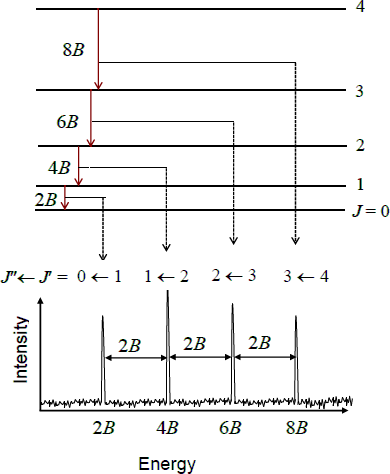
\includegraphics[width=0.5\textwidth]{Rotational_spectrum_example.png}
				\caption{Beispiel-Spektrum von Rotationsübergängen. \cite{WikiRotat}}
				\label{img:bspspektr}
			\end{figure}

	\newpage
	\section{Durchführung}

		Zur Untersuchung der Rotationsbande aus dem Spektrum der Übergänge $\fett{OH}^\ast(\nu=3-1)$ wurde ein Gitterspektrograph benutzt. Dieser ist auf den Bereich der zu erwartenden Wellenlängen zwischen $\unit[1500]{nm}$ und $\unit[1600]{nm}$ kalibriert und feinjustiert. Dessen Computer-gestützter Shutter ermöglicht die Aufnahme von Referenz-Messungen in Form von Dunkelströmen aus dem Array. Diese werden des Weiteren als Korrektur verwendet.\\
		Der Aufbau ist für eine feste, positive Neigung gegen den Horizont im nordwestlichen Himmel orientiert. Eine Einzelmessung beträgt $\unit[15]{s}$, wobei alle $\unit[15]{min}$ ein Dunkelstrom.Spektrum aufgenommen wird. Eine Erhöhung der Genauigkeit wird durch die Integration mehrerer Messungen eines eingeschränkten Zeitraums erreicht. Die verwendeten Daten entstammen den wolkenlosen Nächten des 25.05.2015 (\fett{Spektrum A}) und 19.03.2015 (\fett{Spektrum B}).

	\newpage
	\section{Auswertung}

		\subsection{Simulierte Spektren}

		\subsection{Reale Spektren}

				\begin{align}
					y\ix{i}=\frac{||I\ix{i}-I\ix{0,i}||}{\text{sup}\left\lbrace ||I\ix{i}-I\ix{0,i}||\right\rbrace\ix{i=0}^{N}} \label{eq:norm}
				\end{align}

			Die Abbildung \autoref{img:spektr1} zeigt die erhaltenen Spektren zum  25.05.2015 (\fett{Spektrum A}) und 19.03.2015 (\fett{Spektrum B}) nach Korrektur mit den entsprechenden Dunkelströmen aus dem Array. Der Verlauf des Graphen macht eine qualitative Betrachtung schwer, weswegen eine Glättung nach dem polynomischen Vorbild der \autoref{eq:glatt} vorgenommen wurde. Die sich daran anschließenden Spektren sind demnach jeweils nach \autoref{eq:norm} normiert und geglättet. Dabei entspricht $y\ix{i}$ dem $i$-ten Wert der Intensität zur $i$-ten Wellenlänge.

				\begin{align}
					&y^{(s)}\ix{i}=\frac{y\ix{i-3}+y\ix{i-2}+y\ix{i-1}+y\ix{i}+y\ix{i+1}+y\ix{i+2}+y\ix{i+3}}{7} \label{eq:glatt} \\
					\text{wobei:} \quad &y^{(s)}\ix{1}=\frac{y\ix{1}+y\ix{2}+y\ix{3}+y\ix{4}}{4} \quad \text{usw.} \nonumber\\
					\text{und} \quad &y^{(s)}\ix{N}=\frac{y\ix{N-3}+y\ix{N-2}+y\ix{N-1}+y\ix{N}}{4} \nonumber
				\end{align}

				\begin{figure}[h]
					\centering
					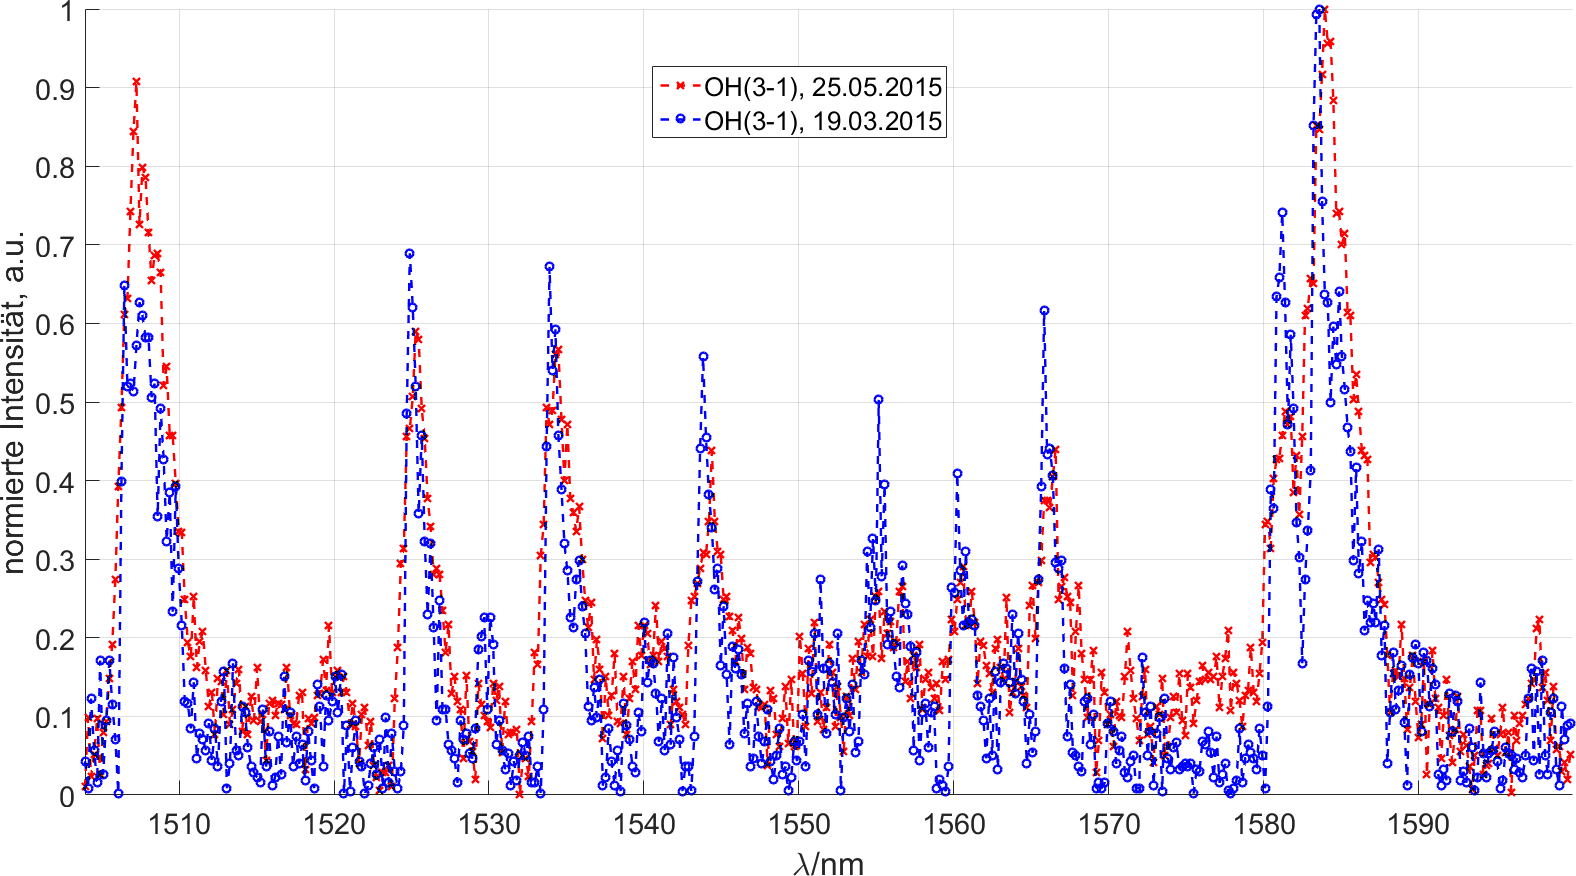
\includegraphics[width=0.9\textwidth]{spektr_unsmooth.png}
					\caption{Betrag der Differenz aus gemessenem Spektrum und Dunkelstrom-Intensität $|I-I\ix{0}|$. Gezeigt sind Verläufe vom 25.05. und 19.03.2015.}
					\label{img:spektr1}
				\end{figure}

			Die \autoref{img:spektr2} zeigt die geglätteten, normierten Messwerte. Insbesondere die Struktur der $P\ix{1}(j)$- und $P\ix{2}(i)$-Peaks, welche nur durch das ungepaarte Elektron unterschieden werden, kann sehr gut beobachtet werden. Jedoch ist durch die Glättung natürlich eine gewisse Einbuße an Peak-Höhe zu verzeichnen, was für die Betrachtung der Rotationsbande aber keine Rolle spielt.\\
			Links und rechts im Spektrum sind deutlich die Maxima der ersten Q-Zweige $\fett{OH}(4-2)$ bzw. $\fett{OH}(3-1)$ zu sehen. Zwischen den hier betrachteten P-Zweigen und dem rechten Rand finden sich die Flachen Linien des R-Zweiges $\fett{OH}(4-2)$. Sogar die Emissionslinie für $P\ix{1}(1)$ kann um $\unit[1600]{nm}$ beobachtet werden.

				\begin{figure}[h]
					\centering
					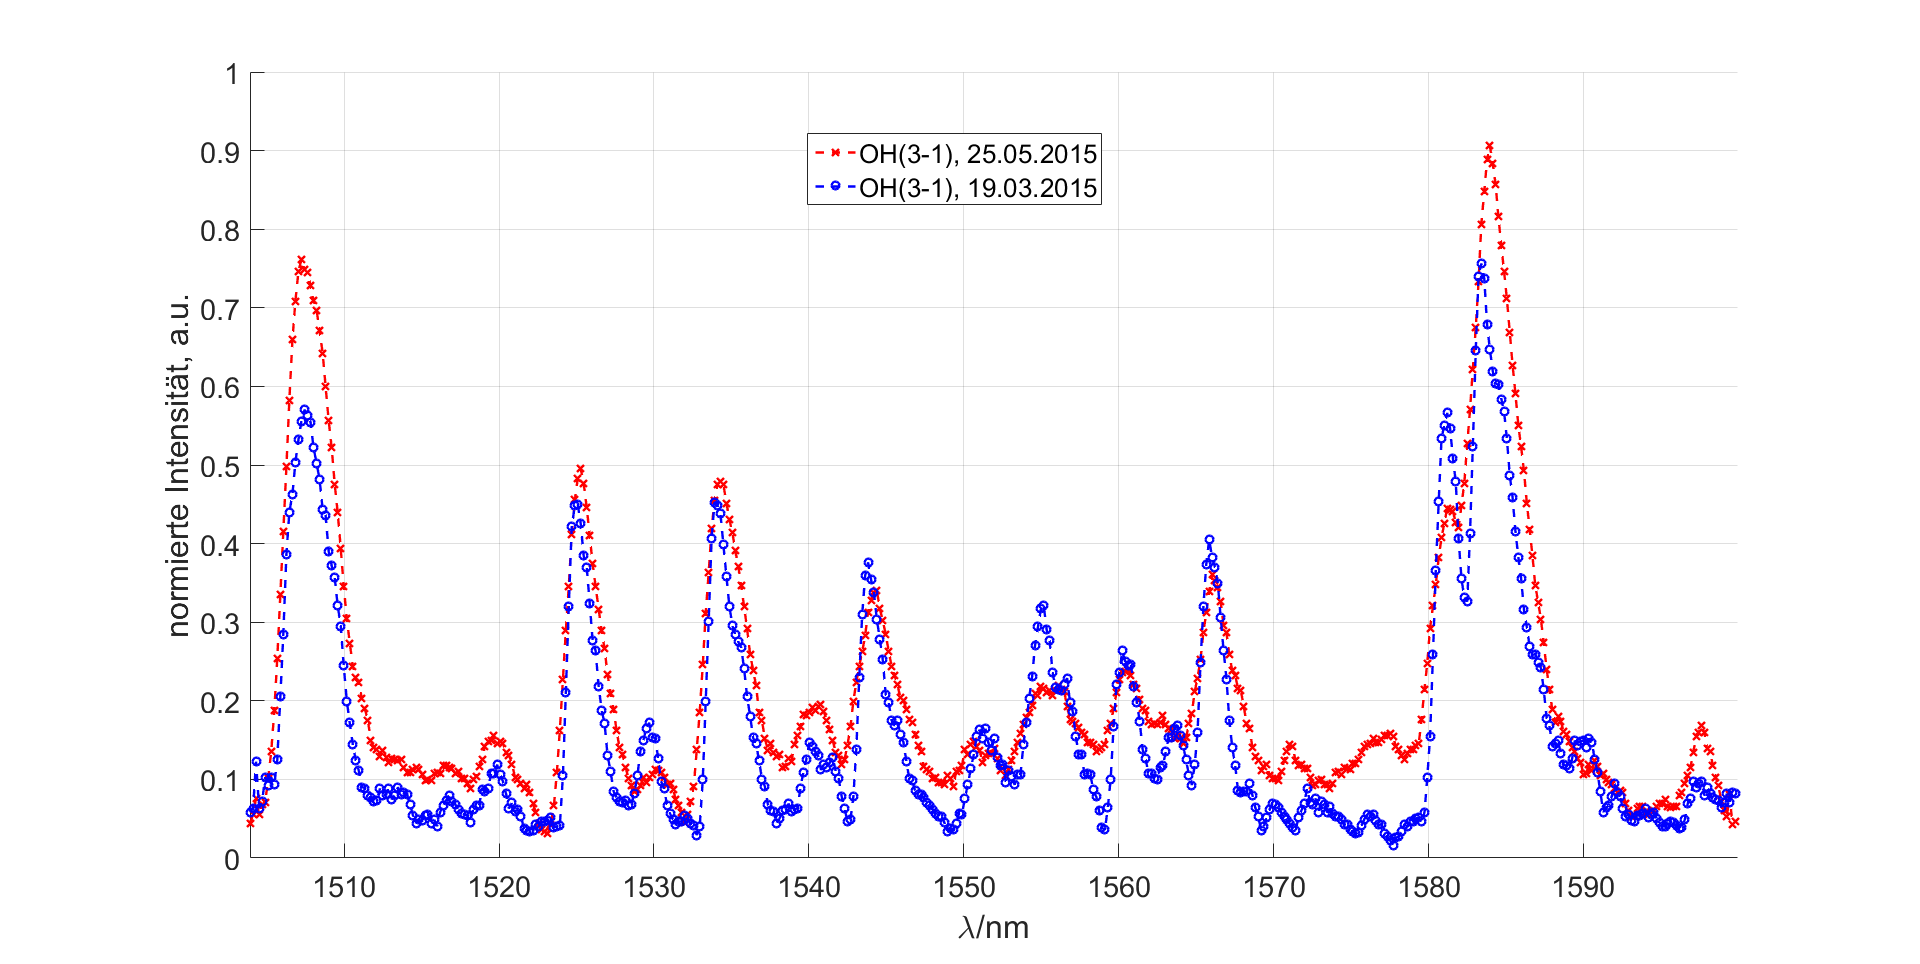
\includegraphics[width=0.9\textwidth]{spektr_smooth.png}
					\caption{Gleiche Daten wie in \autoref{img:spektr1} (Spektrum A, Spektrum B). Hier mit Hilfe einer polynomischen Glättung, maximal der Ordnung 7 verbessert. Der Zusammenhang kommt auf \autoref{eq:glatt}}
					\label{img:spektr2}
				\end{figure}

				\begin{table}[h]
					\centering
					\begin{tabular}{c|c|c|c}
						Peaknummer & $\lambda/\unit[\tenpo{3}]{nm}$, aus \cite{EMAUGreifswaldOHRot} & $\lambda/\unit[\tenpo{3}]{nm}$, A & $\lambda/\unit[\tenpo{3}]{nm}$, B\\
						\hline $P\ix{1}(2)$ & 1,524 & 1,526 & 1,525 \\
						\hline $P\ix{1}(3)$ & 1,533 & 1,535 & 1,534 \\
						\hline $P\ix{1}(4)$ & 1,543 & 1,545 & 1,544
					\end{tabular}
					\caption{Wellenlängen der Peaks $P\ix{1}(2-4)$ im Vergleich zum Literaturwert aus \cite{EMAUGreifswaldOHRot}. Außerdem Gegenüberstellung der Werte aus den Intensitäten zum Spektrum A und B.}
					\label{tab:wellen}
				\end{table}

			Die Positionen der Peaks $P\ix{1}(j)$ der Rotationsübergänge sind in \autoref{tab:wellen} aufgeführt. Deren Intensitäten - ohne Normierung und Glättung, nur nach Korrektur mit Dunkelströmen - finden sich in \autoref{tab:intens}.

				\begin{table}[h]
					\centering
					\begin{tabular}{c|c|c}
						Peaknummer & $|I-I\ix{0}|/\tenpo{2}$, zu A & $|I-I\ix{0}|/\tenpo{2}$, zu B\\
						\hline $P\ix{1}(2)$ & 2,993 & 1,995 \\
						\hline $P\ix{1}(3)$ & 2,873 & 1,945 \\
						\hline $P\ix{1}(4)$ & 2,223 & 1,615
					\end{tabular}
					\caption{Höhen der Peaks $P\ix{1}(2-4)$ an den Positionen aus \autoref{tab:wellen}. Gegenüberstellung von Spektrum A und B. Diese Werte sind für die Auswertung mit der linearen Regression aus \autoref{eq:linreg} wichtig.}
					\label{tab:intens}
				\end{table}

				\begin{figure}[h]
					\centering
					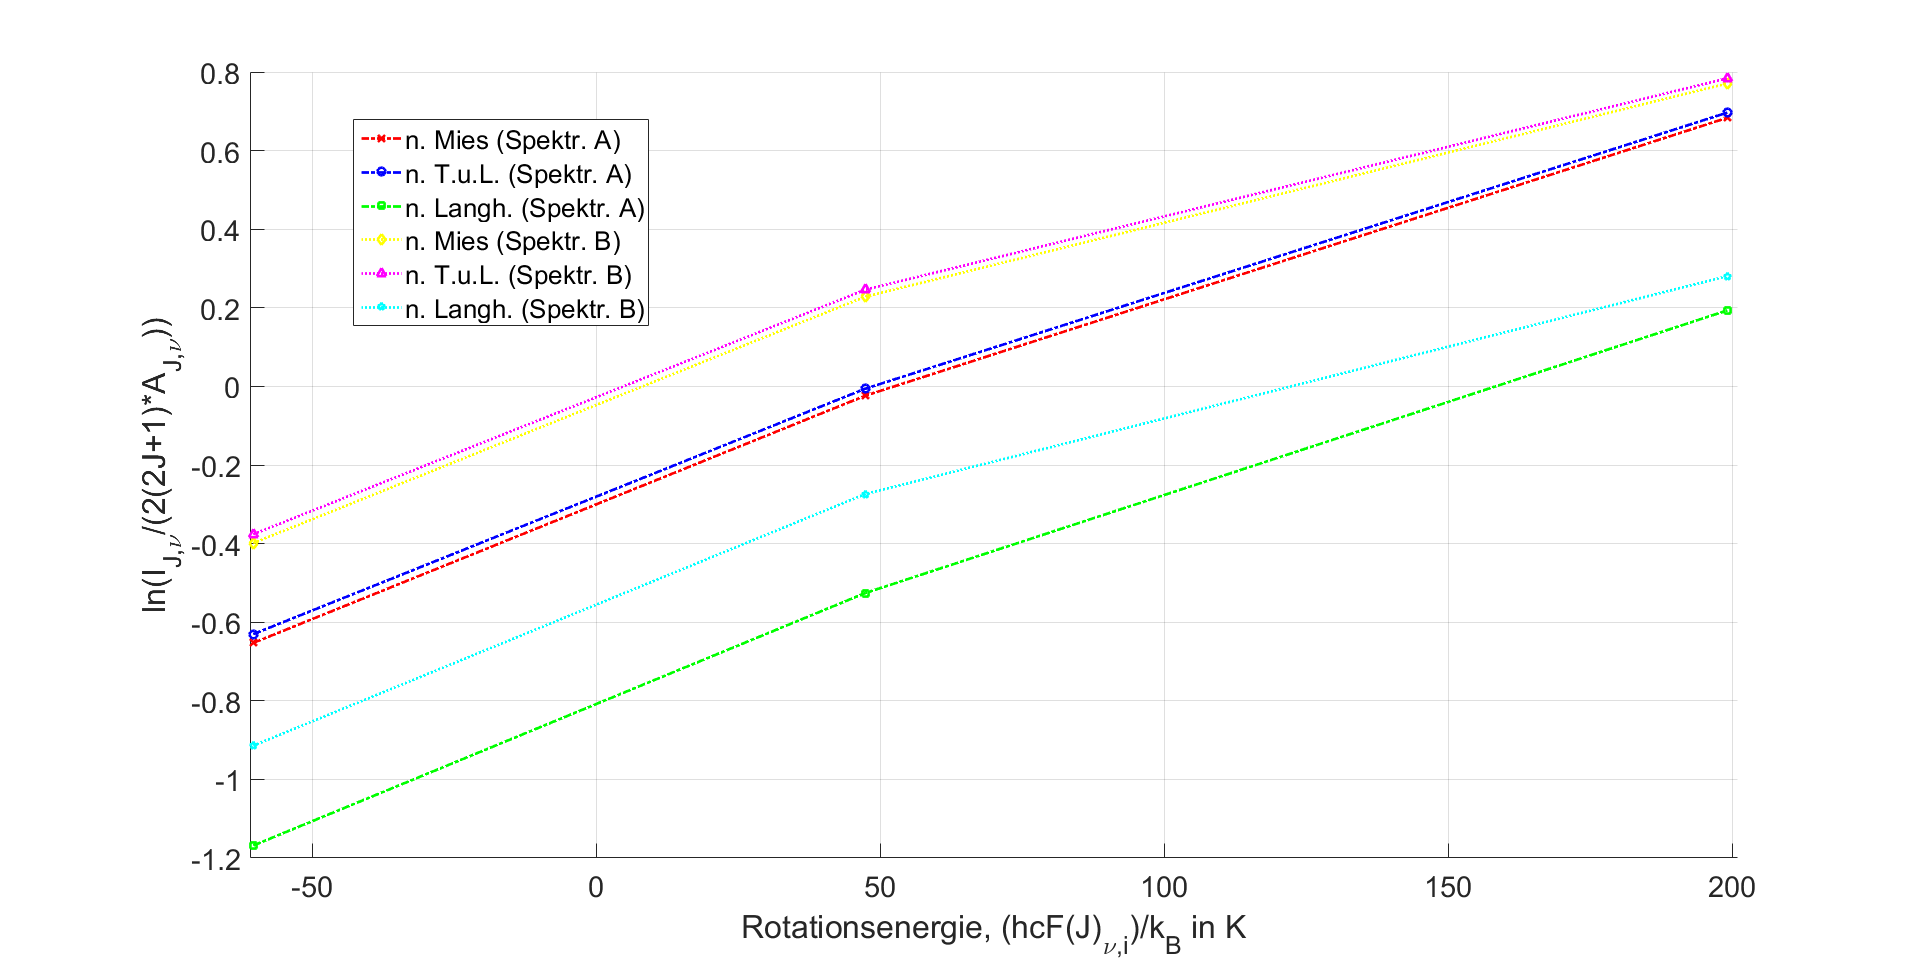
\includegraphics[width=0.9\textwidth]{linear_reg.png}
					\caption{Lineare Regression über die Rotationsenergie und Daten aus \autoref{tab:intens}.}
					\label{img:regress}
				\end{figure}

			Schließlich wurde aus den gemessenen Daten die Rotationstemperatur bestimmt. Dabei gehen die verschiedenen, theoretisch begründeten Einsteinkoeffizienten $A(\lambda\rightarrow\lambda^\prime)$ ein (siehe Mies, Langhoff usw.). Jeweils für Spektrum A und B wurde die lineare Regression nach dem Vorbild aus \autoref{eq:linreg} für 3 verschiedene Übergangswahrscheinlichkeiten durchgeführt. Das graphische Resultat findet sich in \autoref{img:regress}, die daraus erhaltenen Temperaturen in \autoref{tab:trot}.

				\begin{table}[h]
					\centering
					\begin{tabular}{c|c|c}
						Einsteinkoeffizienten, aus \cite{EMAUGreifswaldOHRot} & $T\ix{rot}/\unit{K}$, zu A & $T\ix{rot}/\unit{K}$, zu B\\
						\hline Mies (1947) & 347,98 & 241,75 \\
						\hline Turnbull u. Lowe (1989) & 342,44 & 239,06 \\
						\hline Langhoff (1986) & 1120,1 & 463,93
					\end{tabular}
					\caption{Rotationstemperaturen nach \autoref{eq:linreg}. Die Fehler nach Gauß sind in \autoref{eq:err} angegeben. Für die Intensität wurde das Dunkelstromkorrigierte Spektrum $|I-I\ix{0}|$ benutzt.}
					\label{tab:trot}
				\end{table}

		\subsection{Fehlerrechnung}

%				\begin{figure}
%					\centering
%					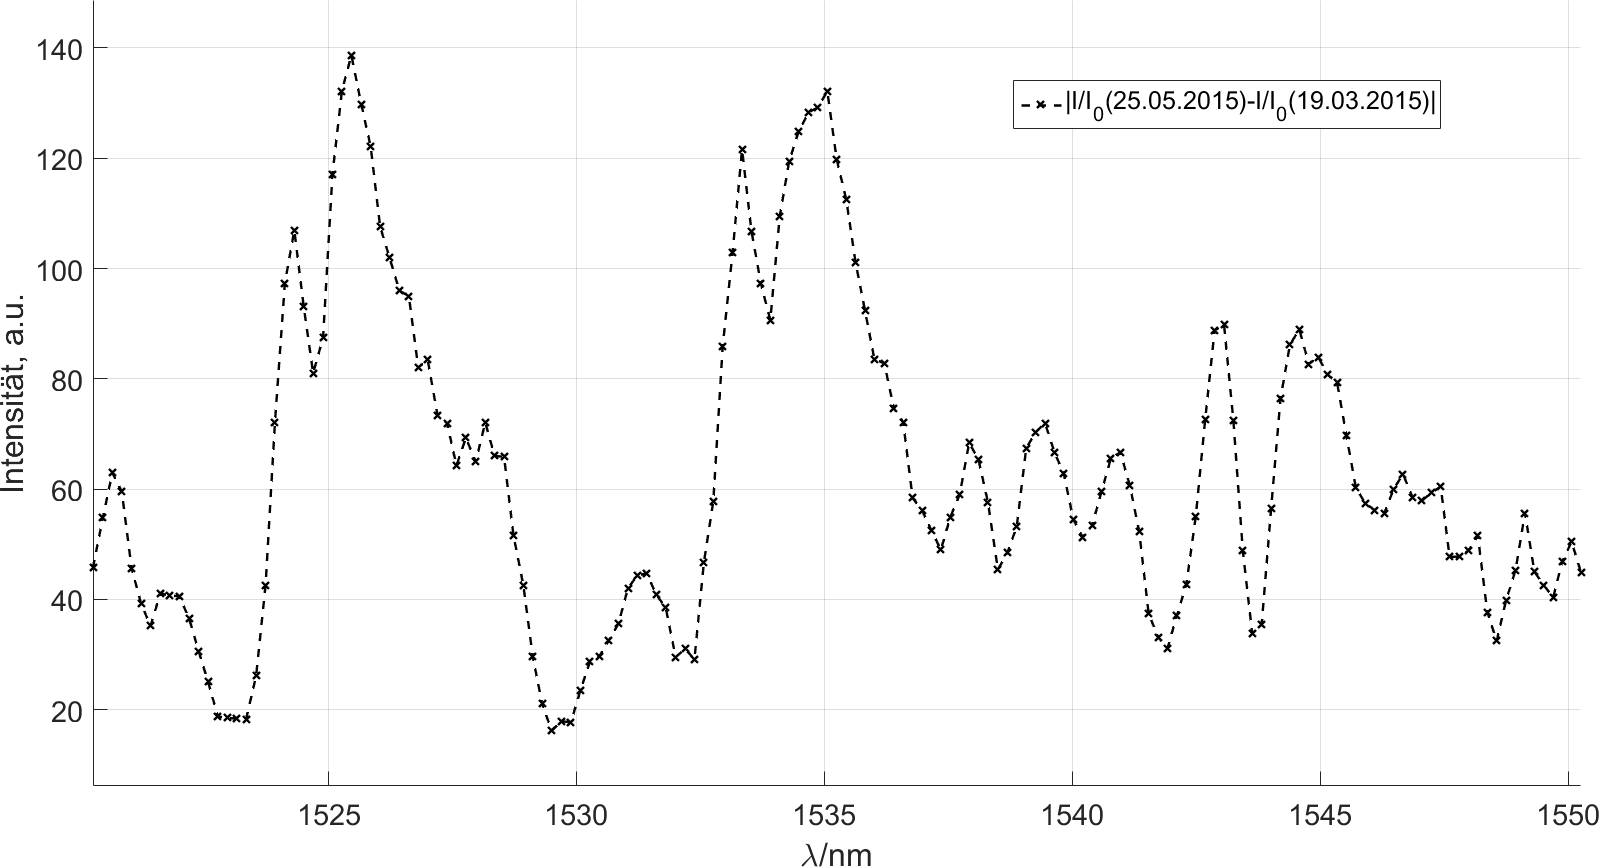
\includegraphics[width=0.9\textwidth]{differenz.png}
%					\caption{Differenz aus Spektrum A und B. Ebenso wie \autoref{img:spektr2} über Polynome geglättet.}
%					\label{img:diff}
%				\end{figure}

			Die in \autoref{tab:trot} berechneten Temperaturen verschiedener Theorien zeigen bereits, welchen Effekt die unterschiedlichen Annahmen über die quantenmechanischen Prozesse der Molekül-Übergänge haben können. Insbesondere die Berechnungen nach Langhoff et. al. weichen sehr stark von den übrigen 2 Werten ab.\\
			Über die Fehlerrechnung nach \tilt{Gauß} aus \autoref{eq:gauss} kann zudem ein weiteres Maß für den Fehler angegeben werden. Dieser ergibt sich, für Spektrum A und B nach Bestimmung der Standardabweichung (nach Maßgabe aus \cite{EMAUGreifswaldOHRotat}), in \autoref{eq:err}. Die Fortpflanzung des Fehlers $\Delta I_{\nu,i,J}$ über die lineare Regression der \autoref{eq:linreg} in den Rotationstemperaturen gibt \autoref{eq:err2} wieder. Für beide Fälle - Spektrum A und B und für die \tilt{gauß'sche} Fehlerfortpflanzung - wurden die Koeffizienten nach Mies benutzt.

				\begin{align}
					T\ix{rot}\left(I,\nu,i,J\right)\propto-&\frac{hcF\left(J,\nu,i\right)}{k\ix{B}}\ln\left(\frac{I\left(\nu,i,J\leftarrow\nu\prime,i\prime,J\prime\right)}{2\left(2J+1\right)A\left(\nu,i,J\rightarrow\nu\prime,i\prime,J\prime\right)}\right)^{-1} \\
					\Delta& T\ix{rot}\approx\sqrt{\left(\frac{\diff T\ix{rot}}{\diff I_{\nu,i,J}}\right)^2\cdot\left(\Delta I_{\nu,i,J}\right)^2} \label{eq:gauss}
				\end{align}

				\begin{align}
					\text{nach Mies:} \quad &T\ix{rot,A}=\left(347,98\pm 0,0424(11)\right)\unit{K} \label{eq:err}\\
					&T\ix{rot,B}=\left(241,75\pm 0,223(22)\right)\unit{K} \nonumber
				\end{align}

				\begin{align}
					\text{nach Mies:} \quad &T^{(A)}\ix{rot,true}\in\left[347,67(03)\unit{K},348,29(02)\unit{K}\right]  \label{eq:err2}\\
					&T^{(B)}\ix{rot,true}\in\left[241,57(63)\unit{K},241,92(90)\unit{K}\right] \nonumber
				\end{align}

	\newpage
	\section{Anhang}

		\bibliography{all.bib}
		\bibliographystyle{unsrt}

\end{document}